\section{Population Study: Characterizing Sub-luminous $\gamma$-Ray Pulsars Using Polarization}
\paperref{This section is based on work done for
``Sub-luminous $\gamma$-Ray Pulsars''
\citep{romani2011sub}}


In the paper ``Sub-luminous $\gamma$-Ray Pulsars'' \citep{romani2011sub} we aimed
to show that pulsars sub-luminous in the $\gamma$-rays
is due to alignment using radio polarization modeling
and data.
The $\gamma$-ray luminosities scales with the spin-down energy as
$L_{\gamma}\approx(\dot{E}\times 10^{33} $ erg/s$)^{1/2}$.
This is based on properties of the Goldreich-Julian model
($L_{\gamma}\propto\dot{E}^{1/2}$, see, for example, \cite{lyne2006pulsar})
plus observation of pulsars \citep{psrcat}.
However, a number of pulsars have luminosity or limits 
that are more than an order of magnitude below this
estimated luminosity, $L_{\gamma}$.
The paper aims to test whether this weak luminosity 
is due to the pulsars beaming away from the Earth.
Other explanations include the pulsars having physical
properties that causes low luminosity or the estimated distance
to the pulsars is drastically off and they are farther away 
than calculated.

\begin{figure}[t!!]
\begin{center}
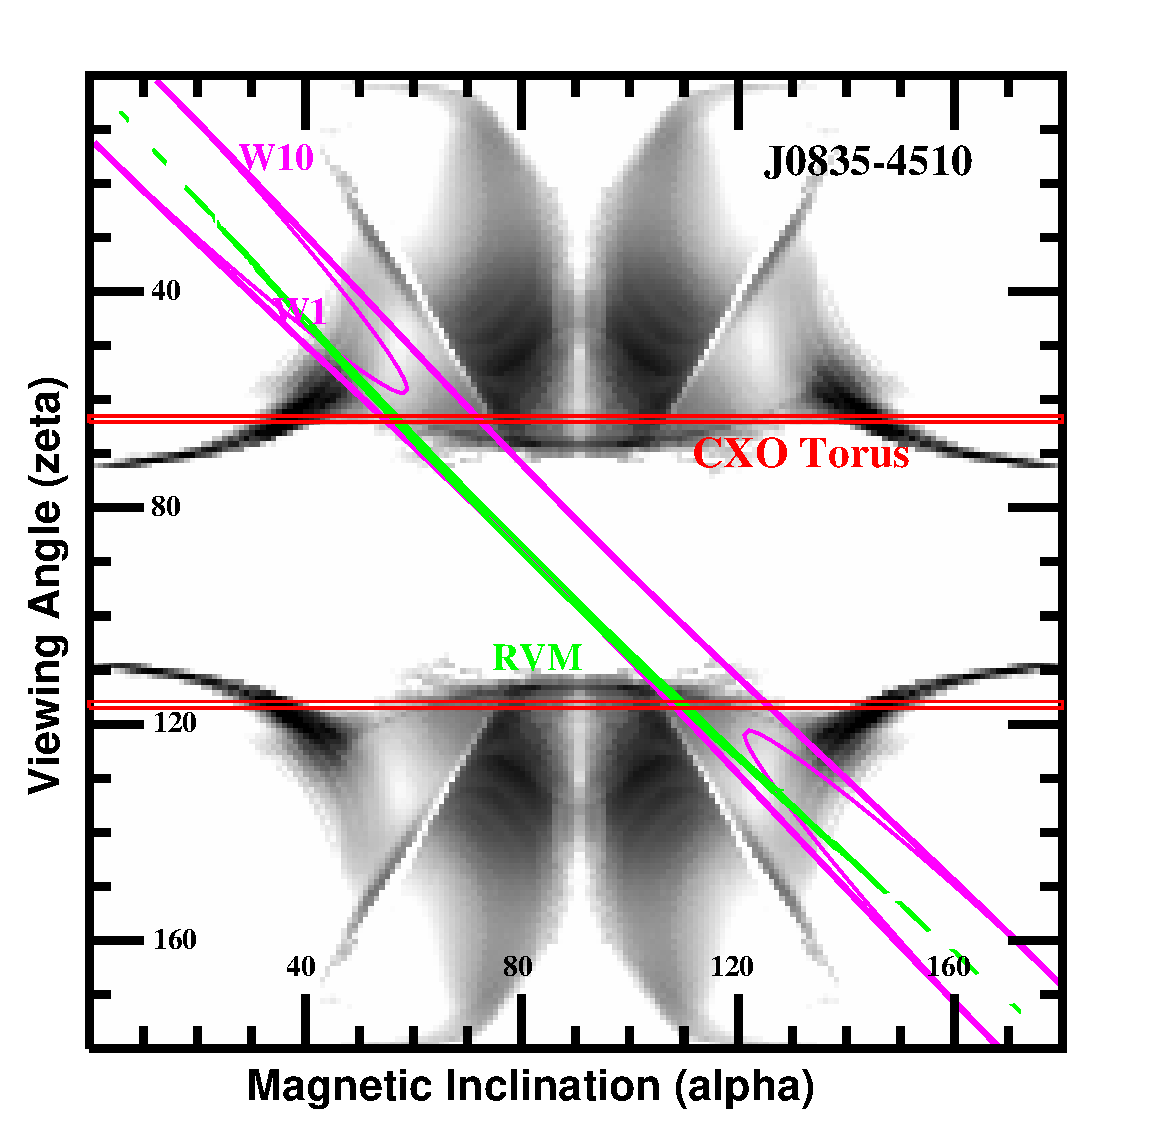
\includegraphics[width=0.5\textwidth]{chapters/multiWaveLength/figures/f2.eps}
\caption[The $\gamma$-ray fit map for Vela in the $\alpha$--$\zeta$ plane with radio polarization, X-ray torus, and pulse width constraints]{
\label{VelaEx} 
Figure taken from \cite{romani2011sub}.
The $\gamma$-ray fit map for Vela in the $\alpha$--$\zeta$ plane with radio polarization, X-ray torus, and pulse width constraints.
The background gray scale shows the goodness of fit of the {\it Fermi} light curve to a
basic outer gap model, with dark colors being better fits. Additionally, red lines mark
constraints from an X-ray pulsar wind nebula torus fit, green contours mark constraints
from RVM, and magenta contours mark constraints from opening angle arguments.
}
\end{center}
\end{figure}


\begin{figure}[htbp]
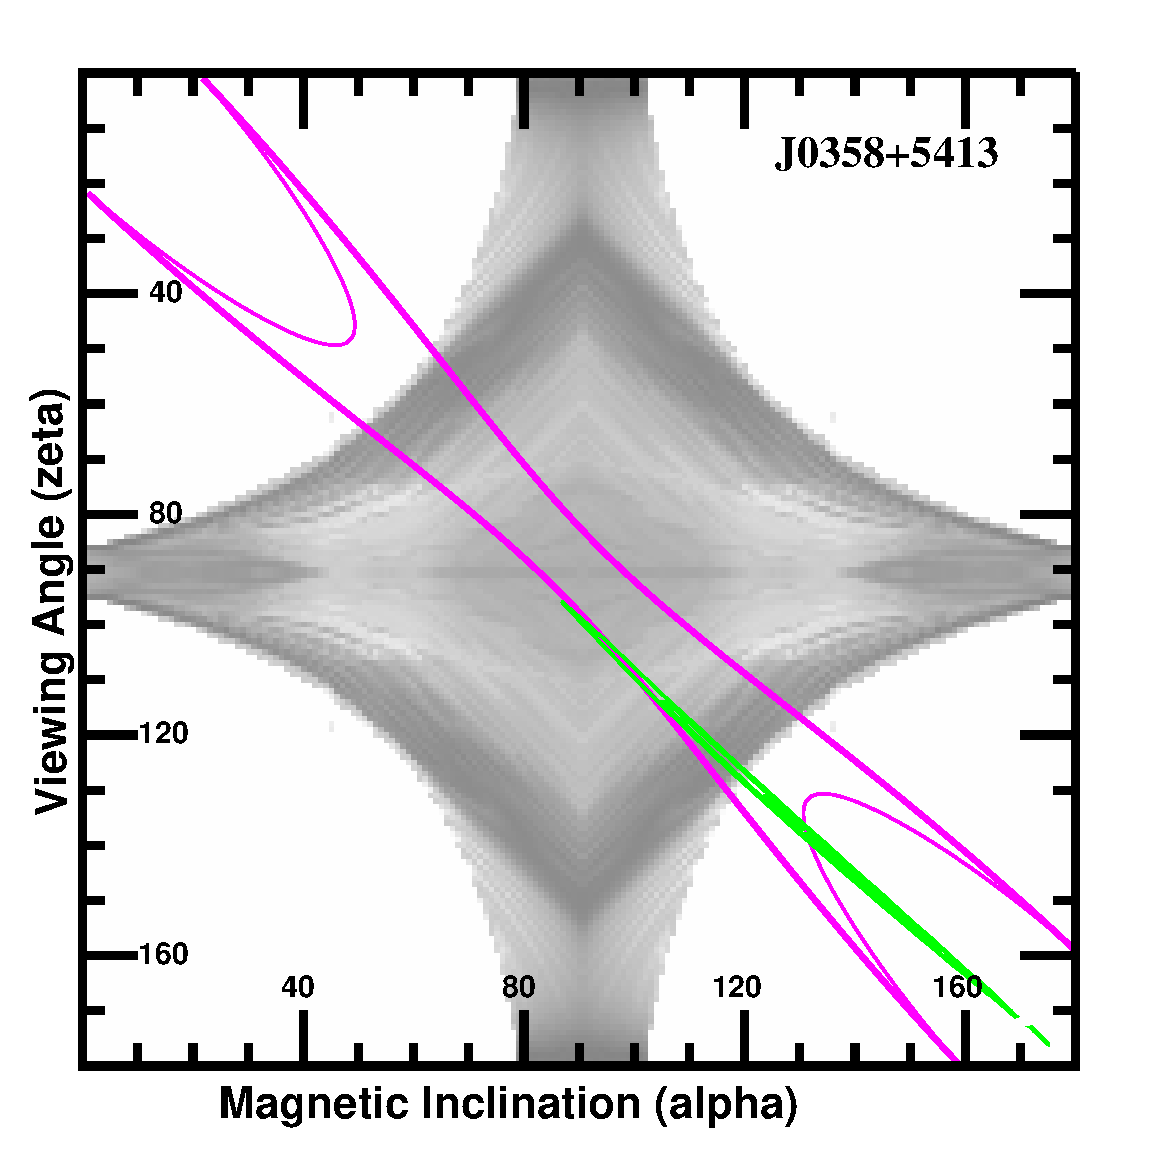
\includegraphics[width=0.5\textwidth]{chapters/multiWaveLength/figures/f3cor_a.eps}
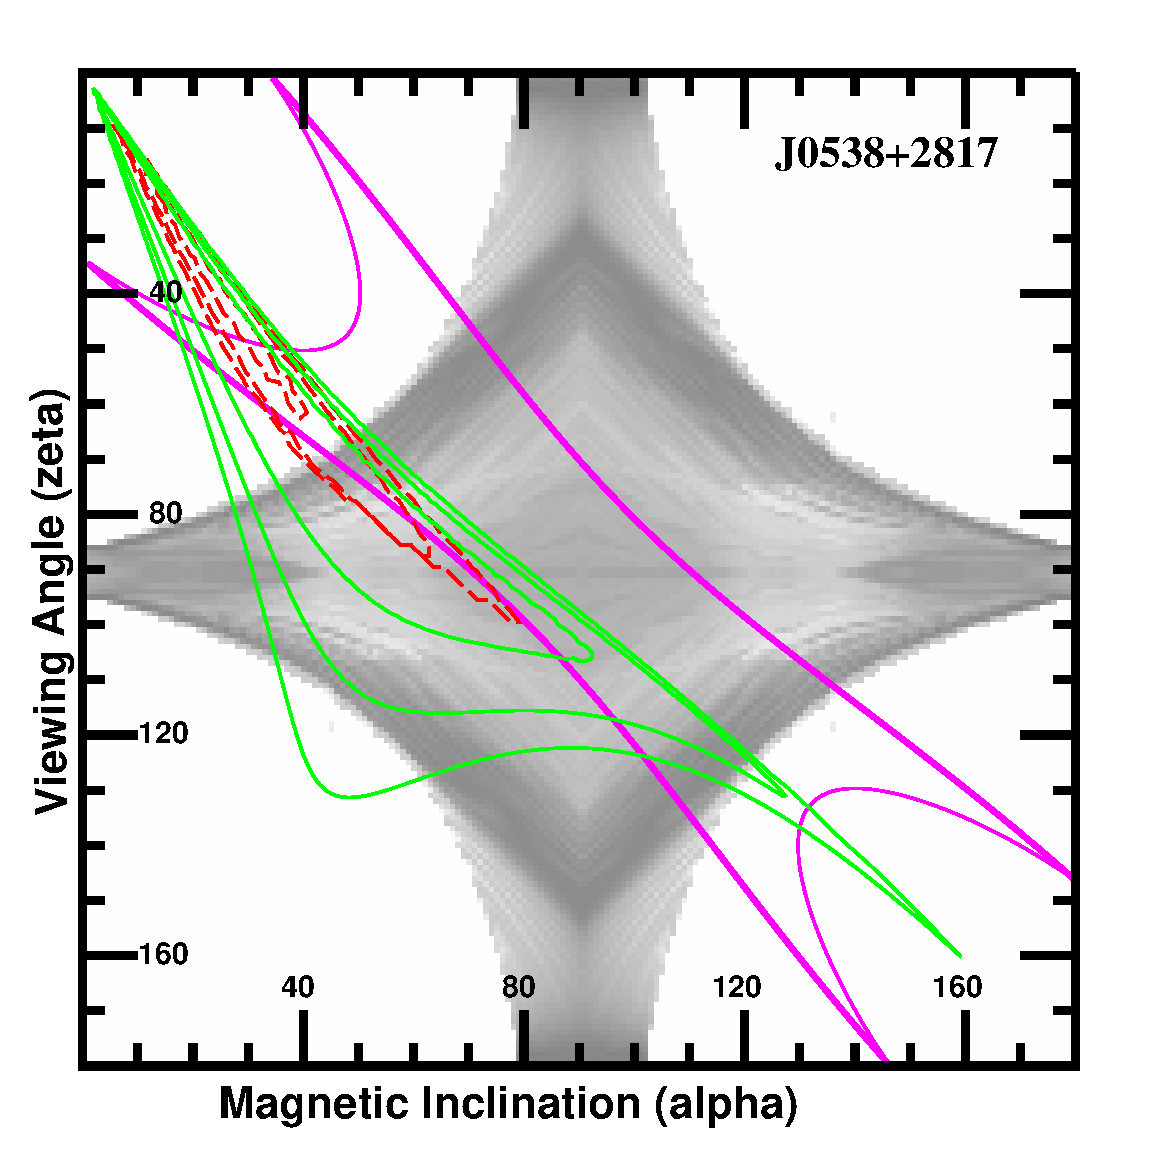
\includegraphics[width=0.5\textwidth]{chapters/multiWaveLength/figures/f3cor_b.eps}
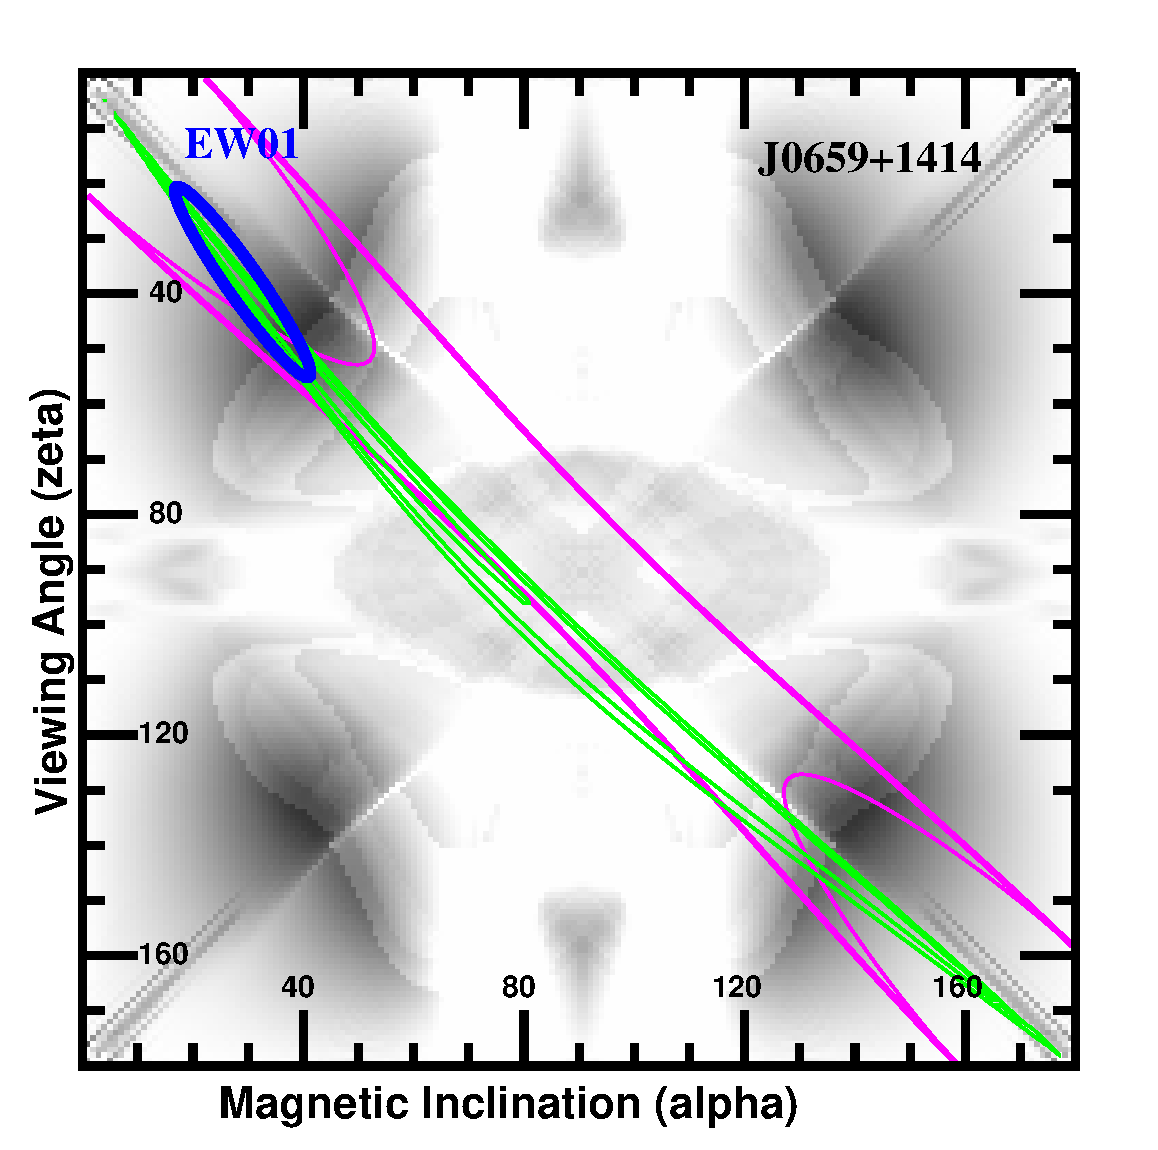
\includegraphics[width=0.5\textwidth]{chapters/multiWaveLength/figures/f3cor_c.eps}
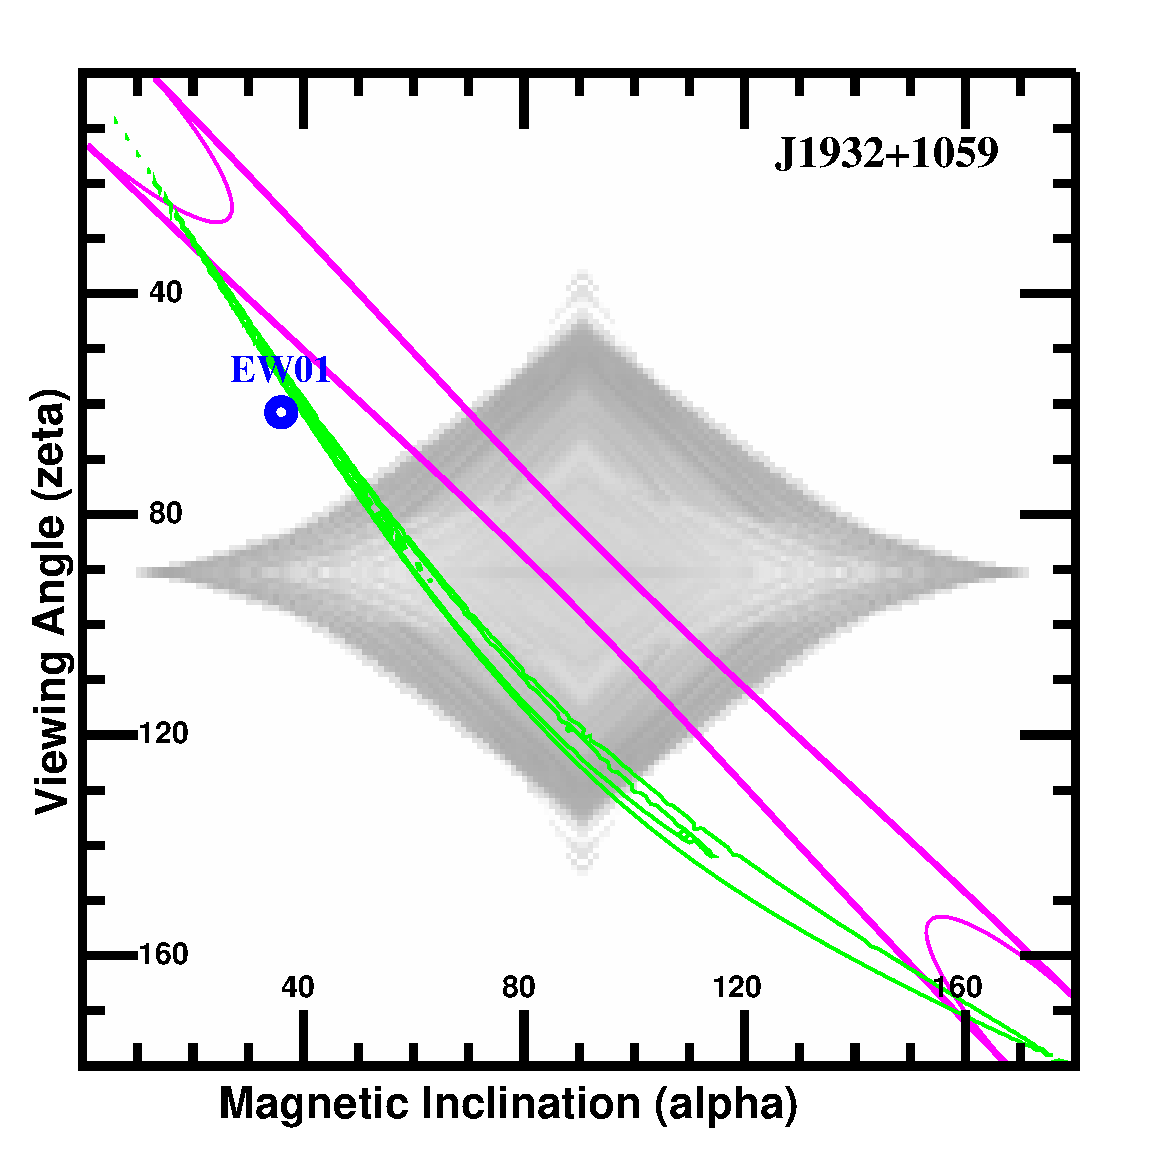
\includegraphics[width=0.5\textwidth]{chapters/multiWaveLength/figures/f3cor_d.eps}
\caption[The $\gamma$-ray fit map for sub-luminous pulsars with parallax
distances in the $\alpha$--$\zeta$ plane with radio polarization and pulse
width constraints]{ \label{plx_const} 
Figure taken from \cite{romani2011sub}.
The $\gamma$-ray fit map for sub-luminous pulsars with parallax 
distances in the $\alpha$--$\zeta$ plane with radio polarization and pulse
width constraints.
The backgrounds show the generic locations providing
sharp outer gap pulses, except for PSR J0659$+$1414, where the background shows the
allowed fits to the observed {\it Fermi} pulses, including lower altitude 
(two-pole caustic model)
%Pole Caustic TPC, Dyks \& Rudak 2003)
emission. 
``Good'' fits here for the other pulsars are in white regions because
of the sub-luminous nature of the pulsars.
Three green contours show the loci of best RVM matches, while the
bold and narrow magenta curves showed the regions allowed by emission from
the static dipole open zone for our estimated emission altitude. For PSR J0659$+$1414 (PSR B0656$+$14)
and PSR J1932$+$1059 (PSR B1929$+$10) the RVM fits of \citet{everett2001emission} are indicated.
For PSR J0538$+$2817 the fits imply large emission altitudes, requiring
a numerical magnetosphere model. The fits to the polarization geometry using
such models are shown by the dashed (red) contours.
}
\end{figure}

\begin{figure}[t!!]
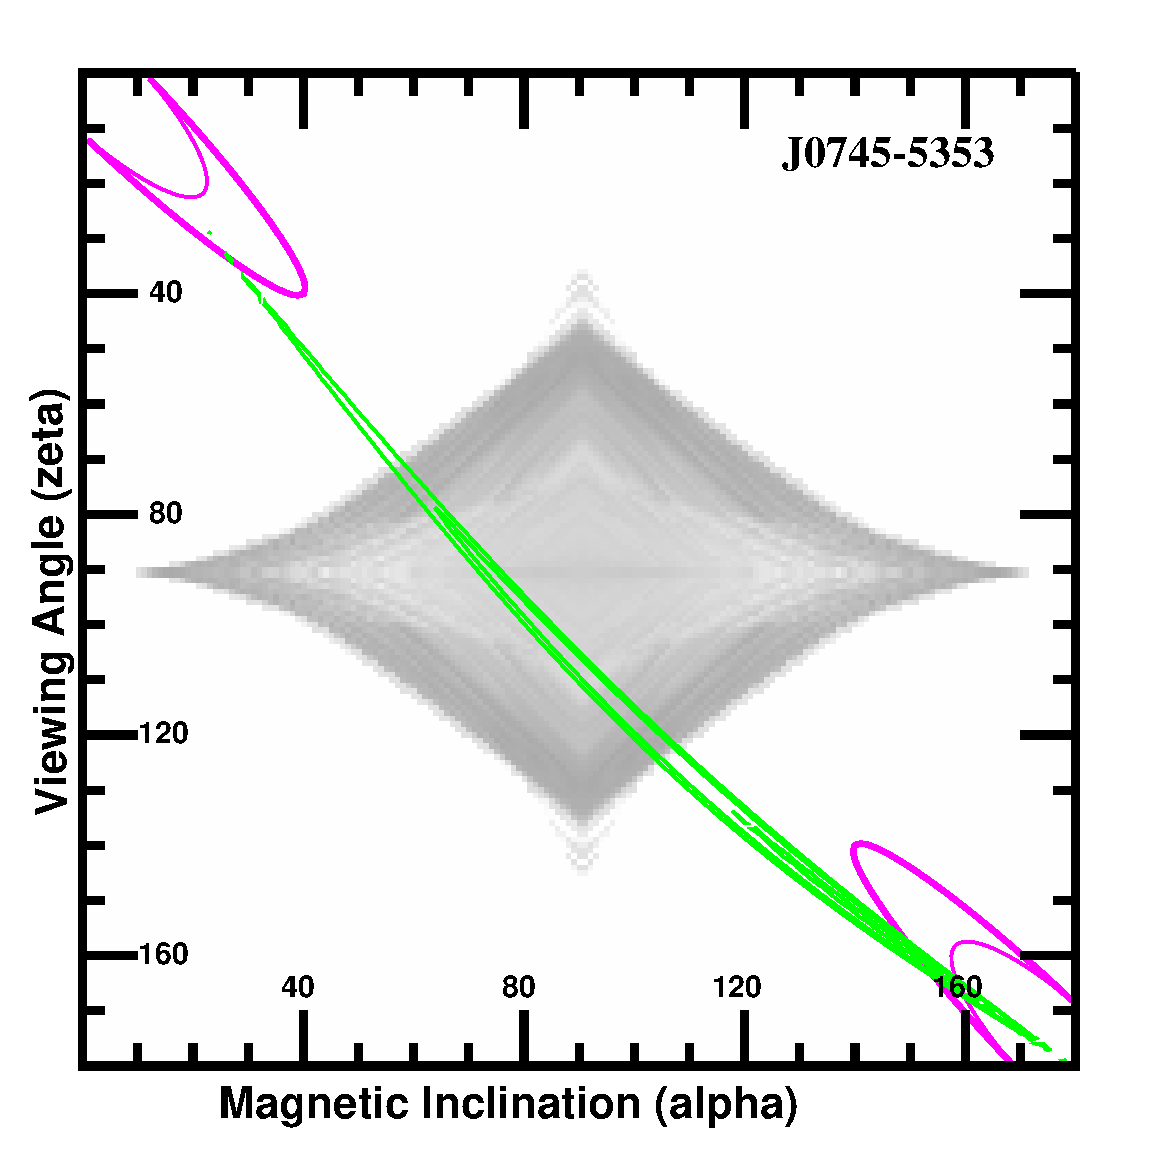
\includegraphics[width=0.5\textwidth]{chapters/multiWaveLength/figures/f4cor_a.eps}
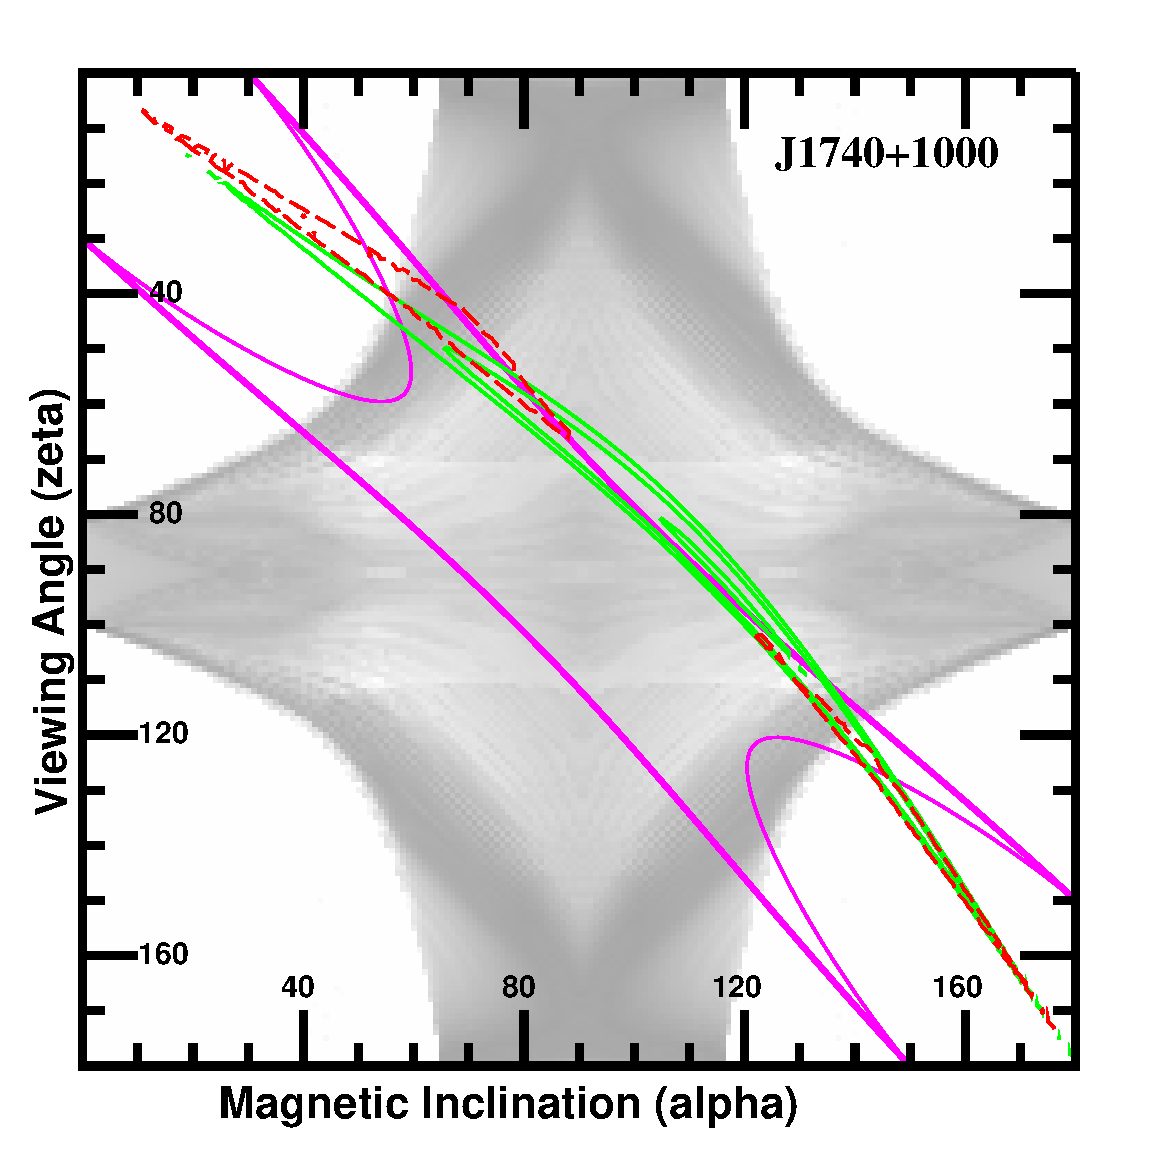
\includegraphics[width=0.5\textwidth]{chapters/multiWaveLength/figures/f4cor_b.eps}
\caption[The $\gamma$-ray fit map for sub-luminous pulsars without parallax 
distances in the $\alpha$--$\zeta$ plane with radio polarization and pulse
width constraints]{\label{noplx_const} 
Figure taken from \cite{romani2011sub}.
The $\gamma$-ray fit map for sub-luminous pulsars without parallax
distances in the $\alpha$--$\zeta$ plane with radio polarization and pulse
width constraints. For geometries
away from the gray background, the sources are not expected to have strong 
outer magnetosphere $\gamma$-ray pulses. 
``Good'' fits here are in white regions because
of the sub-luminous nature of the pulsars.
The PSR J1740$+$1000 data suggest large
emission altitude requiring numerical modeling; the locus of best fits for these models 
is shown by the dashed (red) contours.
}
\end{figure}
Open zone arguments are utilized 
in this paper to constrain acceptable parameter space.  
The parameters $W_1$ and $W_{10}$ represent the
width of the radio pulse assuming that the pulse
ends when the intensity falls below $1\%$ or $10\%$
respectively.  If one definition is more appropriate
for a given pulsar, it will be noted below.
For more details on the relationship between
the phase width and the size of the open zone, 
see Section \ref{sec:beamingGeometry}.

Figure~\ref{VelaEx} is an
example of the use of 
multi-wavelength data to strongly 
constrain the geometry of 
a pulsar.  
The pulsar modeled here is the Vela pulsar (PSR B0833$-$45 or PSR J0835$-$4510).
The pulsar is modeled with $\gamma$-ray data,
radio polarization data, opening angle constraints as
well as X-ray pulsar wind nebula torus fitting 
(see Section \ref{subsec:ToriModeling}).
multi-wavelength data of Vela is used to strongly restricts the possible
parameter space and similar modeling is done for the sub-luminous pulsars.
The magenta contours represent limits
imposed by beaming geometry.  Thin magenta lines represent
$W_{1}$ constant where models with a pulse width
that would accommodate the data are in either corner of the
fitting plane.  For the $W_{10}$ constraint, the models
are limited to those within the thick magenta lines.
The green and red contours show the lowest $\chi^2$ regions
for polarization model fitting.

Unfortunately, none of the other pulsars have clear 
X-ray pulsar wind nebula tori which are strong constraints
on the parameter space.
Four of the pulsars analyzed using polarization have parallax distances available
(PSR J0358$+$5413, PSR J0538$+$2817, PSR J0659$+$1414, and PSR J1932$+$1059) 
and two do not have parallax distances available (PSR J0745$-$5353 and PSR J1740$+$1000).
The fit maps of Figures~\ref{plx_const} and~\ref{noplx_const} show
regions with $\gamma$-ray model gap width of $w\approx L_{\gamma}/\dot{E}$.
The grey background is the fit map of the $\gamma$-ray model to 
a generic single peak pulse except for PSR J0659$+$1414 for which $\gamma$-ray data is
available.  The darker the region, the better the fit.  
Note though that because the pulsars are sub-luminous, the best fit regions
are those that are white regions, since no $\gamma$-rays are present
for these models. 
Blue contours are polarization fit
regions from the literature.  

In the fitting results of PSR J0358$+$5413, the RVM favored $\alpha>110^\circ$.
Additionally, with $W_1$ constraint, $\alpha>130^\circ$ and $\zeta>140^\circ$.
The $W_{10}$ constraints are not more restrictive than the RVM fitting
results.
The pulsar PSR J0358$+$5413 could be sub-luminous but 
some non-sub-luminous geometries are also plausible.

For PSR J0538$+$2817,
the acceptable parameter space given by the
RVM fit is rather large as can be seen in 
Figure~\ref{plx_const}.  However, the combination
of the RVM contours and the $W_{1}$ and $W_{10}$ constraints
are much more restrictive.  With the $W_{1}$ constraint,
the possible models are confined to $\alpha<35^\circ$
and $\zeta<50^\circ$.  The numerical finite-altitude 
fits are included for this pulsar
on the figure in red dashed contours.  These fits
again favor smaller $\alpha$ and $\zeta$ where
one would not expect outer gap emission in $\gamma$-rays.
In contrast, the jet-like feature of the X-ray pulsar
wind nebula does suggest $\zeta\approx90^\circ$
but are too faint to do a formal fit with the torus model
\citep{romani2003pulsar,ng2007origin}.


PSR J0659$+$1414 was previously studied in the radio polarization
\citep{lyne1988shape,everett2001emission,weltevrede2010gamma} 
and the results of \cite{everett2001emission} are included in blue
on the figure.  In our fits to RVM, the model favored $\alpha<80^\circ$
but the pulsar has extended emission well beyond the main peak
such that including the $W_1$ restriction gives $\alpha<35^\circ$.
The goodness of fit given in the figure is for a two-pole caustic
$\gamma$-ray model fit to the {\it Fermi} Large Area Telescope data
available for this pulsar. 
The outer gap model emission best fits are restricted
to $50^\circ<\alpha<130^\circ$ and are well beyond the restrictions
of the strongly extended emission seen in this pulsar.  

The fitting of the polarization data of PSR J1932$+$1059 prefers 
$\alpha<60^\circ$.  However, the additional constraints of 
$W_{10}$ prefers $\alpha<20^\circ$ and $W_{1}$ prefers
$\alpha<15^\circ$.  The RVM fitting contour from
\cite{everett2001emission} is also included on Figure~\ref{plx_const}.
Our analysis would then imply strongly that 
this pulsar is sub-luminous through geometry 
although this pulsar
has a low $\dot{E}$ such that the $\gamma$-ray
emission may have turned off.

PSR J0745$-$5353 does not have a defined parallax distance and
thus can not be definitively categorized as sub-luminous.
From the \cite{cordes2002ne2001} model, the pulsar has a distance
of $0.25$ kpc but a distance of $7.1$ kpc from \cite{taylor1993pulsar}.
The pulsar is sub-luminous if its distance is less than $2$ kpc.
In the combined restriction of RVM and $W_{10}$, $\alpha>150^\circ$
and in the combined restriction of RVM and $W_{1}$, $\alpha>160^\circ$.
Thus if PSR J0745$-$5353 was known to be close enough for detection,
it would be a sub-luminous pulsar.

The pulsar PSR J1740$+$1000 also does not have a parallax distance but
does have a strong dispersion measure distance (Section \ref{sec:interstellarScattering}).  
Both RVM and single-altitude numerical model
fitting was performed on the radio polarization position angle data.
For $W_{10}$ and RVM modeling, $\alpha<70^\circ$ or $\alpha>120^\circ$
is preferred.
For $W_{1}$ and RVM modeling, $\alpha<50^\circ$ or $\alpha>140^\circ$
is preferred.
For $W_{1}$ and single-altitude modeling, $\alpha<30^\circ$ or $\alpha>150^\circ$
is preferred.
So although the pulsar could possibility not be detected due to 
geometry, the parameters are not restrictive enough
to test the model.

In conclusion, this paper attempted to determine whether the non-detection
of these pulsars in the $\gamma$-rays is due to beaming direction
and high altitude emission of the outer gap model.
Although the pulsars all showed evidence of being
sub-luminous due to geometry, none were ruled out
as low-level $\gamma$-ray emitters that will yet be detected
with increased {\it Fermi} Large Area Telescope exposure and pulsed searches.

